\documentclass[twocolumn]{article}
\usepackage{geometry}	%
\usepackage{abstract} %to get email footnotes
\geometry{margin=2cm}	%more visible figures (more place) 
\usepackage[superscript,biblabel]{cite}%superscript citing
\usepackage[utf8]{inputenc}
\usepackage[english]{babel}
\usepackage{amsmath}	%booklet
\usepackage{hyperref}	%clickable citings, referencing URL via \url{}
\usepackage{siunitx}	%for SI units; see ftp://ftp.dante.de/tex-archive/macros/latex/exptl/siunitx/siunitx.pdf
\usepackage{graphicx} 	%includegraphics
\usepackage{mhchem}		%writing chemical elements with mass numbers
\usepackage[nottoc]{tocbibind}	%references
\usepackage{indentfirst}%indenting first paragraphs

%the command \insertFigure{file} inserts figure with width 0.9*(column width)
\newcommand{\insertFigure}[1]{%
   \includegraphics[width=0.95\linewidth]{#1}%
}

\title{\textbf{K223: $\gamma$-$\gamma$ Angular Correlation}}
\author{Bence Mitlasóczki\thanks{s6bemitl@uni-bonn.de} and Beno\^it Scholtes\thanks{s6bescho@uni-bonn.de} \\ \textit{Rheinische-Friedrich-Wilhelms Universit\"at Bonn}}
\begin{document}
\renewcommand{\abstractname}{\vspace{-\baselineskip}} %supresses abstract title
\twocolumn[ %makes a one column abstract
\begin{@twocolumnfalse}
\maketitle
\begin{abstract} \vspace{-8mm}
This paper analyses the angular correlation between subsequent photon emissions in the $\gamma$-$\gamma$ cascade of decaying $\ce{_27^{60}Co}$. A FAST-SLOW coincidence circuit with scintillation detectors, single channel analysers, and constant fraction discriminators were used to measure the number of $\gamma$-$\gamma$ cascade decays for angular separations from 90$^\circ$ to 270$^\circ$. The data was corrected for the measured accidental coincidences. The data was in agreement with the theoretical angular correlation function and its coefficients. The fit coefficient values calculated are $B = 0.116  \pm 0.066 $ and $C = 0.040 \pm 0.075$. The large uncertainty is to be expected from previous experiments though could have been reduced with longer measuring times.
\end{abstract}
\end{@twocolumnfalse}
\hspace{5mm} ]
\maketitle
\saythanks %from abstract package to ensure email footnotes from \thanks command in a two-collumn article
\section{Introduction}
In order to conserve angular momentum, the probability that a nucleus relaxing toward the ground state will emit a photon in a given direction is dependent on the angle between the direction of emission and the spin axis of the nucleus.\cite{sieg} When studying a free nucleus, the nuclear spin axis is free to rotate in space and thus $\gamma$ emissions are isotropic. If relaxation proceeds through successive $\gamma$ emissions however, the two emissions will be angularly correlated if there isn't enough time for the projection of the nuclear spin to be perturbed and rotated by extra-nuclear fields in between the two emissions. The aim of this paper is to verify the angular correlation expected from the $\gamma$-$\gamma$ cascade of decaying $\ce{_27^{60}Co}$. To do so, a FAST-SLOW coincidence circuit was initially set up and the $\gamma$ spectrum of a $\ce{_27^{60}Co}$ sample was measured. The number of angularly correlated photons for different angles were then measured, as well as the number of wrongly counted coincidences. The angular correlation of decaying photons provides us with information on properties of the nucleus and nuclear decay, such as the spin of nuclear levels and the angular momentum carried by radiation. 

\section{Theory}
A detailed treatment of the theory of the angular correlation of nuclear radiation is provided in chapter XIX of \textsl{Siegbahn}.\cite{sieg}
 Figure \ref{fig:cobalt_scheme} shows the decay scheme of the sample used. The $\ce{_27^{60}Co}$ with half-life of $\approx 5.3$ years decays via $\beta^-$-radiation into $\ce{_28^{60}Ni}$ with highest probability to the $4^+$ angular momentum state. $\ce{Ni}$ then relaxes to the ground state with the largest branching ratio being the $4^+\rightarrow2^+\rightarrow 0^+$ decay, producing two $\gamma$ photons with respective energies of 1.17 and 1.33~MeV. The lifetime of the intermediate $2^+$ $\ce{Ni}$ state is on the order of $\SI{1}{\pico\second}$ which is too short to be perturbed by extra-nuclear fields due to Heisenberg's uncertainty principle. The decay of a free $\ce{_27^{60}Co}$ nucleus is thus suitable for the angular correlation treatment.
\begin{figure}[!h]
\centering
\insertFigure{cobalt_scheme.png}
\caption{$\ce{_27^{60}Co}$ decay scheme \cite{cobalt_scheme}.}
\label{fig:cobalt_scheme}
\end{figure}
\par As the direction of the emission of the first photon is encoded with information on the projection of the spin axis of the nucleus due to angular momentum conservation, the probability of the direction of emission of the second photon depends on the direction of the first emission. Thus, there is an angular correlation between the directions of the two $\gamma$ emissions, given by the following directional correlation function for the $\gamma$-$\gamma$ cascade herein considered:
\begin{equation}
W(\theta) = 1+A_{22}P_2(\cos{\theta})+A_{44}P_4(\cos{\theta}), \label{eq:corr}
\end{equation}
where $P_2$ and $P_4$ are Legendre Polynomials, $A_2 = 0.1020$, and $A_4 = 0.0091$.\cite{sieg} This is the relation that will be tested in this paper.
\newpage

\section{Experimental setup}
The design of the apparatus is shown in Figure \ref{fig:exp_setup}. 
\begin{figure}[!h]
	\centering
	\insertFigure{k223_setup.png}
	\caption{Experimental setup\cite{booklet}.}
	\label{fig:exp_setup}
\end{figure}
The slow circuits count the number of photons incident to the respective detectors which have energies within energy ranges set by the respective single channel analysers. This circuit is used to only count the number of incident $\gamma$~photons with energies from the relevant $\gamma$-$\gamma$ cascade. The fast coincidence circuit counts the number of pairs of photons which arrive at the two detectors within a time window set by the fast coincidences unit. This circuit is used to distinguish and count pairs of photons which come from single $\gamma$-$\gamma$ cascade events as opposed to pairs of photons from two different cascade events. Though some random coincidences are still inevitably measured due to the large number of $\gamma$-$\gamma$ cascade events occurring at a given time in the $\ce{_27^{60}Co}$ sample, these random coincidences are eventually accounted for as will be discussed in Section~\ref{sec:acc}. The number of coincident photons from the fast and slow circuits are then matched by the universal coincidence unit to count the number of pairs of photons with the right energies and within the right time frame to be labelled as coming from single $\gamma$-$\gamma$ cascade events.
\begin{figure}[!h]
	\centering
	\insertFigure{pmt.png}
	\caption{Scintillation detector with photomultiplier\cite{pmt}.} 
	\label{fig:pmt}
\end{figure}
\subsection{Detector}
The detectors consist of a crystal scintillator and a photomultiplier as show in Figure~\ref{fig:pmt}. The scintillator absorbs the $\gamma$-ray and re-emits visible light in form of scintillation, which induces electron emission in the photomultiplier (\textbf{PMT}) via the photoelectric effect. The high voltage provided between the photo-cathode and the anode accelerates the electron, which induces an avalanche of electrons by colliding with each of the dynodes. The signal produced by the \textbf{PMT} has a measurable height which is proportional to the energy of the incident photon. This signal is then input to the constant fraction discriminator in the fast circuit to measure the arrival time of the incident photon. As this procedure distorts the signal shape, which is required for the measurement of the energy of the incident photon, the output pulse cannot be used to measure the energy. Instead, an undistorted signal from an earlier phase of the amplification process is used as the input for the single channel analyser (\textbf{SCA}) in the slow circuit.
 \begin{figure}[!h]
 	\centering
 	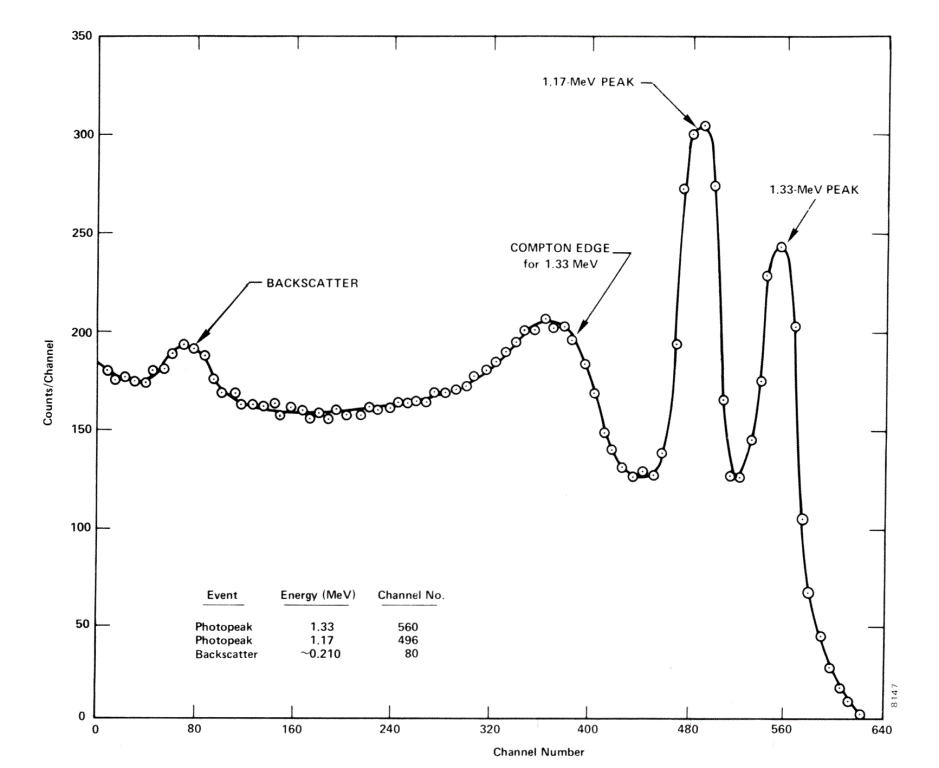
\includegraphics[width=1\linewidth]{Compt.png}
 	\caption{Compton scattering in the $\ce{^{60}Co}$ $\gamma$-$\gamma$ cascade spectrum\cite{Compt}.} 
 	\label{fig:Compt}
 \end{figure}
\par One should note that Compton scattering also occurs in the scintillator when incident photons scatter inelastically inside the crystal instead of being absorbed. Scintillation photons are then produced with lower energy than those produced via absorption. This creates a Compton plateau spectrum bordered by two peaks on either side, as seen in Figure~\ref{fig:Compt}. The Compton edge is caused by the photons backscattering in the crystal, depositing the maximum of energy in the crystal from Compton scattering. The backscattered peak is instead caused by photons scattering back into the detector from the lead casing of the detector, with a large loss of energy, and then being absorbed by the crystal.\cite{Compton} Though Compton scattering distorts the measure energy spectrum, the peaks from the absorbed photons should still be easily discernible at higher frequencies, visible in Figure~\ref{fig:Compt}.


\subsection{Constant Fraction Discriminator}
%The fast coincidence circuit checks whether the two detected photons come from the same decay process. 
The constant fraction discriminators modify the signals as seen in Figure~\ref{fig:cfd}. An attenuated inverted copy of the input is added to the delayed input signal. The resulting shape crosses the $\SI{0}{\volt}$ line, called the ``zero crossing point". This point serves as a time stamp for the signal which does not depend on the amplitude of the signal. The discriminator has two outputs: the ``fast" output which is a negative digital pulse and the ``slow" output which is a positive one. The latter was used as this is the one needed for the fast coincidence unit \textbf{FC}.
\begin{figure}[!h]
	\centering
	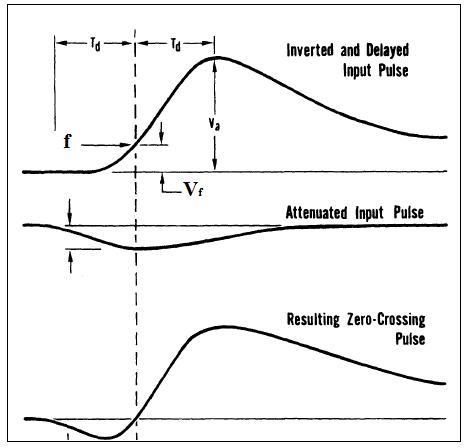
\includegraphics[width=0.95\linewidth, height=0.7\linewidth]{cfdnew.png}
	\caption{Constant fraction discriminator operation\cite{cfd}.} 
	\label{fig:cfd}
\end{figure}

\subsection{Single Channel Analysers}
The weak, undistorted detector signal coming from the \textbf{PMT} is fed through the amplifiers \textbf{A1} and \textbf{A2} first. The analysers \textbf{SCA1} and \textbf{SCA2} determine whether the amplitudes of the signals, which are proportional to the energy of the detected $\gamma$~photons, fall into an interval set by the \textbf{SCA}s. The interval is over a range of so-called channels of the \textbf{SCA} which are set either with upper and lower limit channels or with a lower limit and a window size.

\subsection{Universal coincidences}
The output signals from the \textbf{SCA}s and the \textbf{FC} are sent to the universal coincidence unit \textbf{UC} to count the total number of coincident photons within a time span set by the timer. The signals from the \textbf{SCA}s are first sent through delays to make sure the signals incident to the \textbf{UC} correspond to photons hitting both detectors at the same time. The output from the \textbf{FC} is fed to a gate $\&$ delay generator \textbf{D$^2$-G$^2$} which delays the fast signal to ensure that the fast coincidences are correctly assigned to the same photons measured in the slow circuit when fed into the \textbf{UC}. Thus, the \textbf{UC} counts the total number of pairs of photons which have the right energies, and arrive within a short enough time frame, that is expected from $\gamma$-$\gamma$ cascade events.


\section{Procedure} \label{sec:Proc}
\subsection{Solid Angle Corrections}
Solid angle correction factors $Q_2$ and $Q_4$ for detectors placed 5, 7, and 10~cm from the $\ce{^{60}Co}$ sample are provided by the literature.\cite{sieg} These factors correct for the limiting assumption made by the angular correlation function Equation~\ref{eq:corr} that the detectors are point-like. The closer the detectors are placed to the source, the larger the solid angle of the detectors become and thus the uncertainty introduced from the fact that they do not simply measure counts for a single angle is increased. That said, the further away the detectors are placed from the source, the smaller the photon count rate becomes for a given time span which increases the relative uncertainty of the count rate (as photon emissions follow Poisson statistics). Rough measurements were taken for different detector placements to estimate the expected uncertainty introduced by photon counts for the angular correlation measurements. It was decided to place the detectors 7~cm away from the source in order to minimise uncertainty, though whether this is indeed the best placement cannot be known due to the unknown nature of the uncertainty introduced by the solid angle correction. As the solid angle correction factors depend on the energy of the incident photons and correction factors are only known for energies of 0.5, 1.0, and 1.5~MeV, linear interpolation was utilised to obtain factor values for the $\gamma$-$\gamma$ cascade photons which have energies of 1.17 and 1.33~MeV and thus a mean of $E_{\text{avg}} = 1.252$~MeV. The factor values obtained from the linear interpolation are,
\begin{align*}
&Q_2\big(E_{\text{avg}}\big) \equiv Q^*_2 = 0.9623,\\
&Q_4\big(E_{\text{avg}}\big) \equiv Q^*_4 = 0.8782.
\end{align*}
This method reduces the uncertainty caused by the energy dependence of the solid angle correction factors. That said, there remains a small uncertainty caused by the different energies of the two cascade photons which would require individual correction factors. We do not distinguish between the two different cascade photons during measurements in this experiment however.

\subsection{Amplifiers and CFDs}
The amplifiers \textbf{A$_1$} and \textbf{A$_2$} were then adjusted. We changed the gain using an oscilloscope such that the peaks corresponding to different detected photon energy levels didn't hit the $\SI{9}{\volt}$ output ceiling of the amplifiers. We set the maximum to approximately $\SI{8}{\volt}$. The result of the adjustment is shown in Figure \ref{fig:amp}. Next we set the threshold of the constant fraction discriminators above the noise level by using the output of the \textbf{CFD} as the trigger for the amplifier signal of the same detector. We increased the threshold until the bright line at $\SI{0}{\volt}$ showing noise disappeared. This was done to make sure that the \textbf{CFD} only triggered for detected photons.
\begin{figure}[!h]
	\centering
	\insertFigure{./screenshots/SC08_cropped.png}
	\caption{Well-adjusted signal of the first amplifier. A too high gain would cause the highest peaks to flatten due to saturation before the maximum.} 
	\label{fig:amp}
\end{figure}

\subsection{Prompt Curve}
We connected the positive outputs of the \textbf{CFD}s to the fast coincidence unit \textbf{FC}, one of them through a delay unit \textbf{D3}. While keeping the resolution time of the \textbf{FC} at $\SI{15}{\nano\second}$, which was a value approximately expected, we changed the delay of \textbf{D3} to measure the coincidental detections as a function of the delay. We measured the counts for $\SI[separate-uncertainty = true]{10.0(1) }{\second}$ for each delay value which was sufficient to plot an informative prompt curve, given in Figure~\ref{fig:prompt}. From the figure, the count rate approximately plateaus from a delay of approximately 4~ns to 18~ns. This gave confidence in the resolution time of the \textbf{FC} of $\SI{15}{\nano\second}$, and thus this was the chosen value for the angular correlation measurements. That said, a more careful investigation follows immediately below. We set the delay of \textbf{D3} to 11~ns, in the middle of the plateau. The Gaussian fitted post factum confirmed our choice for the delay ($\mu$), yet provided an experimental resolving time of the \textbf{FC} of $\text{FWHM} = 2 \sqrt{2 \text{ln}2} \sigma = \SI[separate-uncertainty = true]{21.9 \pm 3.0}{\nano \second}$,\cite{signal} which is in disagreement with our chosen resolving time. Here one must consider the numerous error sources of this calculated width. Firstly, the theoretical prompt curve is a rectangle\cite{leo} whereas the smoothened edges are attributed to time jitter caused by the imperfection of the electronic components, such as generated pulses which are not perfectly rectangular. If one wants to read off the resolution time, defined as the FWHM of the prompt curve, one needs to take this jitter into account. Thus even though the Gaussian is not the theoretical shape, it can be used more easily and yields a more precise result than taking the length of the plateau.\cite{leo} Secondly, there exists a constant background, caused by the accidental coincidences (two atoms radiate at the same time). This is clearly visible if one considers the fitted Gaussian at $>60$~ns values, where it gives a count of $<10^{-4}$ while the measurements yield approximately 20 counts. Ultimately, the calculated FWHM is known to be uncertain and thus further experiments should aim to obtain a more accurate value to determine a more appropriate resolution time. A shorter resolution time of 15~ns was used meaning that some coincidences were not measured. This should not affect the angular correlation data however, merely the quantity of data, and thus has not introduced uncertainty.
\begin{figure}[!h]
	\centering
	\insertFigure{prompt.png}
	\caption{The measured prompt curve and a fitted Gaussian to quantify the width. The parameters are $\mu = \SI[separate-uncertainty = true]{11.1 \pm 0.9}{\nano\second}$ (mean), $\sigma = \SI[separate-uncertainty = true]{9.3 \pm 1.3}{\nano\second}$ (deviation), $A = 8259.8 \pm	881.8$ (scaling factor). Two measured values at 61~ns ($17 \pm 4.1$ counts) and 63~ns ($29 \pm 5.4$) are not shown, yet quantify accidental coincidences.}
	\label{fig:prompt}
\end{figure}

\subsection{Energy Spectra}
The energy spectra from both detectors was plotted by scanning the entire relevant channels of both \textbf{SCA}s. The detectors were placed at 180$^{\circ}$ separation where the largest number of coincidence counts are theoretically expected. We again measured the counts for $\SI[separate-uncertainty = true]{10.0(1) }{\second}$ which was sufficient to obtain adequate spectra. A window size of 150 channels for both \textbf{SCA}s was used. Measurement were taken until the full spectrum expected from Figure~\ref{fig:Compt} was obtained for both detectors. The spectra are given in Figure~\ref{fig:spectra}.
\begin{figure}[!h]
	\centering
	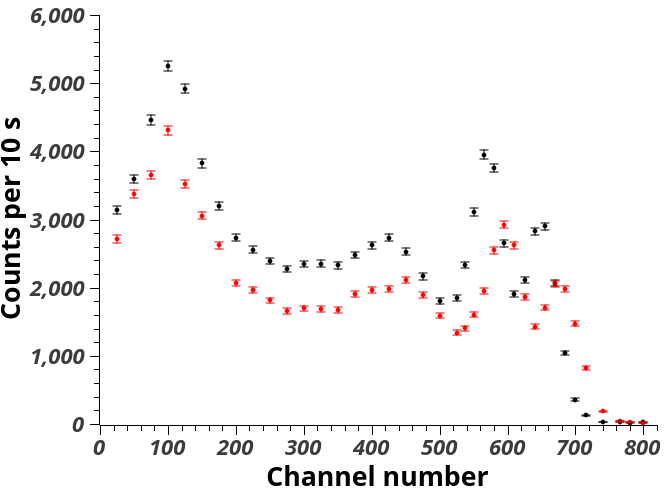
\includegraphics[width=0.9\linewidth]{detectors3.png}
	\caption{Measured energy spectra of both detector 1 (fixed during the experiment, black) and 2 (red).}
	\label{fig:spectra}
\end{figure}
The two $\gamma$-$\gamma$ cascade photon peaks are clearly visible for both detectors at the upper end of the spectra, as well as the backscatter peaks at the lower end of the spectra and Compton edges around channel 450. The channel windows chosen for \textbf{SCA1} and \textbf{SCA2} were 520--720 and 540--740 respectively, in order to include both $\gamma$-$\gamma$ cascade photon peaks.
\par The horizontal shift visible between the two spectra is a constant factor due to the different calibrations of the two detector systems. Using the channel number as units, the first peak appears at $565 \pm 15$ and $595 \pm 15$ for detector one and two, respectively. From this, $\alpha = 0.950 \pm 0.035$ results as the value for detector 1 divided by the value for detector 2. Similarly, we detect the second peak for detectors 1 and 2 at $655 \pm 15$ and $670 \pm 15$, respectively, yielding $\alpha = 0.978 \pm 0.031$, suggesting that the two spectra are indeed offset by a constant factor. The difference in the number of counts for the two spectra instead suggests a difference in the efficiencies of the two detectors. Both of these offsets should not introduce uncertainty in the experimental results.

\subsection{SCA Delays}
The delays of the two \textbf{SCA}s, \textbf{D1} and \textbf{D2}, needed to be individually set to coincide with the \textbf{FC} unit when fed into the \textbf{UC}. 
\begin{figure} [!h]
	\centering
	\insertFigure{./screenshots/SC07_cropped.png}
	\caption{Adjusting the delay of the \textbf{SCA}s such that the leading edges of the signals from one \textbf{SCA} (yellow) and the \textbf{FC} unit (blue) coincide.}
	\label{fig:sca-overlap}
\end{figure}
Both \textbf{SCA}s were separately connected to the oscilloscope with the \textbf{FC}, which was set as the trigger. The leading edges of the rectangular digital signals of the \textbf{SCA} and the \textbf{FC} were aligned using the oscilloscope as the \textbf{UC} uses these leading edges when counting coincidences. This is shown for the first \textbf{SCA} in Figure~\ref{fig:sca-overlap}.

\subsection{Accidental Coincidences} \label{sec:acc}
Though the \textbf{UC} unit ensures to count a coincidence only when a pair of photons with the right energies are detected within an adequately short enough time frame, this still means that two different atoms decaying at the same time are counted as a coincidence when detected. These accidental coincidences were accounted for by measuring them overnight for $\SI{59820}{\second}$ to determine how many of the angular correlation counts were instead accidental coincidences and could be subtracted. This was done by setting the \textbf{D$^2$-G$^2$} delay to its maximum setting to make sure that only coincidences from two different atoms were being counted. A total of $21855 \pm 148$ coincidences were recorded, which corresponds to $146.14 \pm 0.99$ counts over $\SI{400}{\second}$ and $0.3653 \pm 0.0025$ counts each second. The individual \textbf{SCA} units measured $(260560 \pm 16)\times 10^3$ and $(243720 \pm 16)\times 10^3$ incoming photons, corresponding to
 \begin{equation}
 N_{\text{SCA 1}} = 4355.73 \pm 0.27 \hspace{8pt} \text{and} \hspace{8pt} N_{\text{SCA 2}} =  4074.22 \pm 0.26 \nonumber
 \end{equation}
 counts each second. Using the time resolution $\sigma = \SI[separate-uncertainty = true]{21.9 \pm 3.0}{\nano \second}$ of the \textbf{FC} from Figure~\ref{fig:prompt}, we calculated the expected accidental coincidences to be\cite{leo}
%without superscript: (see \cite{leo} for a detailed explanation) as ...
\begin{equation}
N_{\text{acc}} = \sigma \cdot N_{\text{SCA 1}} \cdot N_{\text{SCA 2}} = 0.389 \pm 0.053 \nonumber
\end{equation}
counts per second, which is in good agreement with the experimental results.

\section{Results}
\subsection{Angular Correlation}
Table~\ref{tab:data} presents the angular correlation measurements. 
\begin{table}[htbp]
	\centering
	\begin{tabular}{c||c|c||c|c}
		\hline
		\textbf{Angle} & \textbf{UC} & \textbf{UC-norm.} & \textbf{UC -- acc.} & \textbf{Unc.} \\ \hline \hline
		90    & 5,576 & 3717  & 3,571 & 61 \\ \hline
		110   & 3,837 & 3837  & 3,691 & 62 \\ \hline
		130   & 3,892 & 3892  & 3,746 & 62 \\ \hline
		150   & 4,102 & 4102  & 3,956 & 64 \\ \hline
		170   & 4,222 & 4222  & 4,076 & 65 \\ \hline
		180   & 6,331 & 4221  & 4,075 & 65 \\ \hline
		200   & 4,165 & 4165  & 4,019 & 65 \\ \hline
		220   & 4,085 & 4085  & 3,939 & 64 \\ \hline
		240   & 3,807 & 3807  & 3,661 & 62 \\ \hline
		260   & 3,797 & 3797  & 3,651 & 62 \\ \hline
		190   & 4,306 & 4306  & 4,160 & 66 \\ \hline \hline

	\end{tabular}%
			\caption{Data for the total universal counts \textbf{UC} at each angle for their respective measuring times mentioned below. These were normalised to 400 seconds (\textbf{UC-norm.}) and lastly corrected for accidental counts (\textbf{UC-acc.}) with propagated uncertainty.} 
	\label{tab:data}%
\end{table}%
We took measurements from 90$^{\circ}$ to 270$^{\circ}$ to span a large range of angles to obtain a more accurate weighted fit and also to test whether the angular correlation relation is indeed symmetric about 90$^{\circ}$. If not, it would suggest that the $\ce{^{60}Co}$ is not exactly in the centre of both detectors (or that the relation is inappropriately applied to this experiment). Spanning a larger range of angles can partially offset errors introduced from a sample not perfectly in the centre. The theoretical function is adapted with the solid angle corrections from Equation~\ref{eq:corr} to
\begin{equation}
W(\theta) = A \big(1 + B (Q^{*}_2)^2 \cos^2 \theta + C (Q^{*}_4)^2 \cos^4 \theta \big), \label{eq:fit}
\end{equation} 
with theoretical $B$ and $C$ values\cite{sieg}
\begin{align*}
&B_{\text{th}} = \frac{1}{8} = 0.125,\\
&C_{\text{th}} = \frac{1}{24} = 0.041\bar{6}.
\end{align*}
$A$ is a simply scaling factor which depends on the measuring time. As the function is a linear combination of $\cos^2$ and $\cos^4$, a more accurate fit is obtained from more precise values on and adjacent to the expected peaks and troughs, while making sure there are sufficient values measured in between them. As a result, the angular correlation counts at the trough and peak expected at 90$^{\circ}$ and 180$^{\circ}$ respectively were measured longer for 600 seconds each while other measurements were taken approximately every 20$^{\circ}$ for 400 seconds. 
\begin{figure} [!h]
	\centering
	\insertFigure{angular.png}
	\caption{Angular correlation with fit (red) and theoretical function (blue) with the theoretical coefficients $B_{\text{th}}$ and $C_{\text{th}}$, and the experimentally calculated value for scaling factor $A$.}
	\label{fig:angular}
\end{figure}
Table~\ref{tab:data} provides the data normalised to 400 seconds. The table also includes the total coincidence counts corrected by the accidental coincidences normalised to 400 seconds by subtracting them. As photons follows Poison statistics, the uncertainty in all counts measured is simply the square root of the count. The uncertainty in the angles was 1$^\circ$ as a result of the imprecision of the apparatus. We fitted the measured data to Equation\ref{eq:fit} using the least-squares-fit method, which produced
\begin{align*}
&A = 3602 \pm 40,\\
&B = 0.116  \pm 0.066,\\
&C = 0.040 \pm 0.075.
\end{align*}
These values are in agreement with the theoretical values expected, given above. That said, the uncertainties in the fit values are quite large, especially for $C$, though this was also found in previous experiments.\cite{meliss} To obtain results with smaller uncertainties and a more precise fit, longer measurement times would be required. A plot of the data with the weighted fit is given in Figure \ref{fig:angular}. A polar plot is provided in Figure~\ref{fig:polar} to aid visualisation of the angular correlation. Both of these figures, in addition to the calculated coefficient values of the fit, suggest that the angular correlation function given by Equations~\ref{eq:corr} and~\ref{eq:fit} are accurately applicable to the $\gamma$-$\gamma$ cascade of decaying $\ce{_27^{60}Co}$.
\begin{figure}[h!]
	\centering
	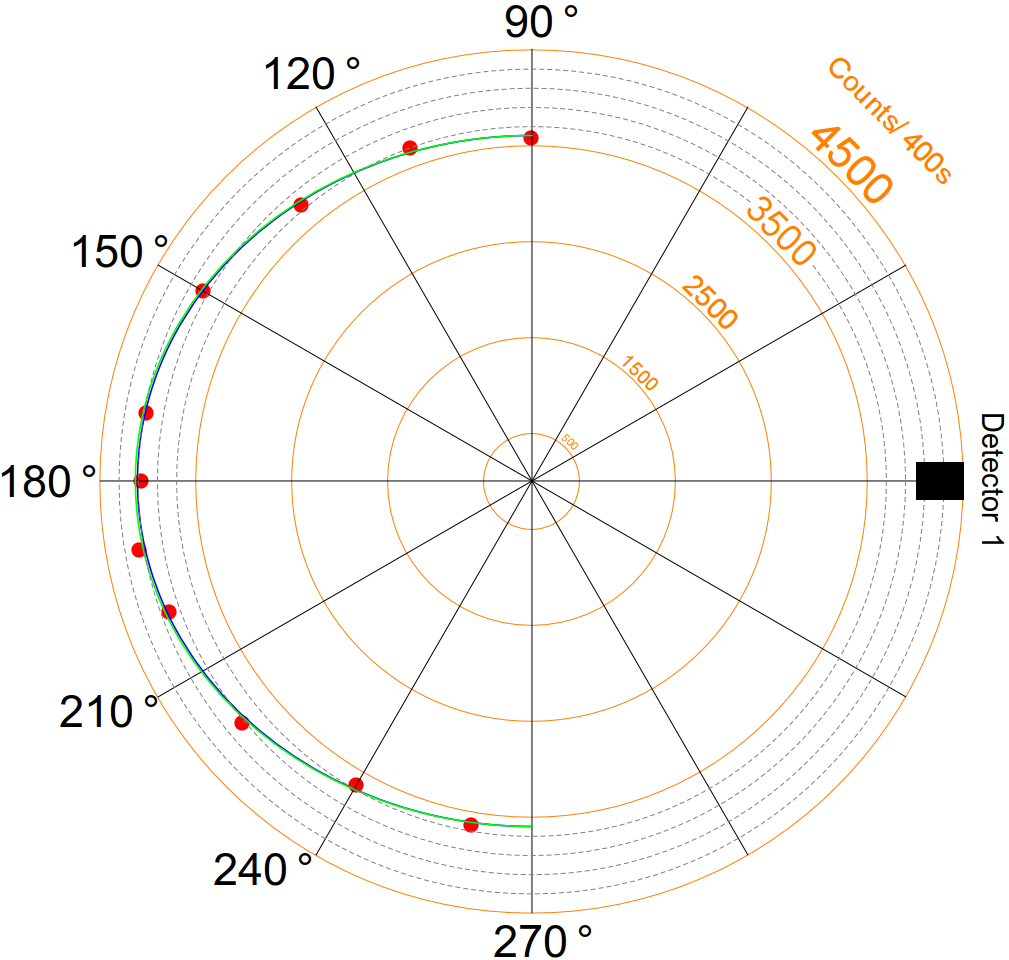
\includegraphics[width=\linewidth]{polar2.png}
	\caption{Polar plot of the counts against angle. Uncertainties are not displayed for the measurements. The weighted fit is given in blue, the theoretical result in green.}
	\label{fig:polar}
\end{figure}

\section{Conclusion}
We set up an experiment to analyse the angular correlation of the $\gamma$-$\gamma$ cascade in a $\ce{_27^{60}Co}$ sample. First we measured the prompt curve which, due to short measurement times and the limited accuracy of a Gaussian fit, resulted in choosing a sub-optimal resolution time for the \textbf{FC} unit. Later experiments should aim to use a more accurate resolution time by performing the prompt curve analysis prior to the angular correlation measurements. Next, we found the relevant energy windows of the two \textbf{SCA}s in order to include both $\gamma$ photon peaks of the $\ce{_27^{60}Co}$ cascade. This was done by finding the individual detector energy spectra, achieved by scanning through the channels of the \textbf{SCA}s. The spectra matched our expectations as they contained the Compton edge, backscattered peak, and the two decay $\gamma$ peaks. The angular correlation measurements of the cascade were then taken and corrected for by measuring also the accidental coincidences. The results obtained are in good agreement with the theory though large uncertainties suggest that the experiment could have benefited from longer measuring times.

\begin{thebibliography}{9}
\bibitem{sieg}
K. Siegbahn, \textsl{Alpha-, beta-, and gamma-ray spectroscopy, Vol. 2} (North Holland Publishing Company, Amsterdam, 1965).
\bibitem{cobalt_scheme}
R. B. Firestone, \textsl{Table of Isotopes $8$\textsuperscript{th} edition} (Wiley, New York, 1996).
\bibitem{booklet}
Unspecified author, \textsl{Advanced Laboratory Course (physics601): Description of Experiments} (University of Bonn, 2018).
 \bibitem{pmt}
 W. U. Boeglin, \textit{Scintillation Detectors}, WWW Document, \url{http://wanda.fiu.edu/teaching/courses/Modern_lab_manual/scintillator.html}.
 \bibitem{Compt}
 Nuclear Power, \textit{Compton Edge}, WWW Document,
\url{https://www.nuclear-power.net/nuclear-power/reactor-physics/interaction-radiation-matter/interaction-gamma-radiation-matter/compton-scattering/compton-edge}.
\bibitem{Compton}
Unspecified author, \textit{Gamma Ray Spectroscopy} (University of Florida, 2013), \url{https://www.phys.ufl.edu/courses/phy4803L/group_I/gamma_spec/gamspec.pdf}.
\bibitem{cfd}
E. Ermis and C. Celiktas, International Journal Of Instrumentation Science 1, (2013), pp.54-62.
%alternative url: https://en.wikipedia.org/wiki/Constant_fraction_discriminator
\bibitem{signal}
M. Nakhostin, \textsl{Signal Processing for Radiation Detectors} (John Wiley $\&$ Sons, 2018), p. 298\footnote{Relevant pages (chapter 6) available for preview under\\ \url{https://books.google.de/books?id=Lrg4DwAAQBAJ}}.
%Mohammad Nakhostin
\bibitem{leo}
W. R. Leo, \textsl{Techniques for Nuclear and Particle Physics Experiments} (Springer-Verlag, 1987), p. 305.
%William R. Leo
\bibitem{meliss}
A. C. Melissinos, J. Napolitano, \textsl{Experiments in Modern Physics, 2\textsuperscript{nd} edition} (Academic Press, San Diego, 2003), pp 419-21.
\end{thebibliography}
\end{document}